% TD-IR Method Framework (LaTeX TikZ/PGF)
% Compile with: xelatex method_framework.tex
\documentclass[tikz,border=6pt]{standalone}
\usepackage{fontspec}
\setmainfont{Times New Roman}
\usepackage{tikz}
\usetikzlibrary{shadows.blur,arrows.meta,positioning,fit,calc}

\definecolor{stagebg}{HTML}{F6F8FA}
\definecolor{stagebd}{HTML}{98A2B3}
\definecolor{keybg}{HTML}{EEF2FF}
\definecolor{keybd}{HTML}{6366F1}
\definecolor{procbg}{HTML}{ECFEFF}
\definecolor{procbd}{HTML}{06B6D4}
\definecolor{okbg}{HTML}{ECFDF5}
\definecolor{okbd}{HTML}{10B981}
\definecolor{warnbg}{HTML}{FFF7ED}
\definecolor{warnbd}{HTML}{F59E0B}
\definecolor{failbg}{HTML}{FEF2F2}
\definecolor{failbd}{HTML}{EF4444}

\tikzset{
  stage/.style={rounded corners=4pt, draw=stagebd, fill=stagebg, line width=0.8pt, align=left, inner sep=6pt},
  key/.style={rounded corners=4pt, draw=keybd, fill=keybg, line width=1pt, align=left, inner sep=6pt},
  proc/.style={rounded corners=4pt, draw=procbd, fill=procbg, line width=0.8pt, align=left, inner sep=6pt},
  ok/.style={rounded corners=4pt, draw=okbd, fill=okbg, line width=0.8pt, align=left, inner sep=6pt},
  warn/.style={rounded corners=4pt, draw=warnbd, fill=warnbg, line width=0.8pt, align=left, inner sep=6pt},
  fail/.style={rounded corners=4pt, draw=failbd, fill=failbg, line width=0.8pt, align=left, inner sep=6pt},
  >={Stealth[length=3mm,width=2mm]},
  flow/.style={-Stealth, line width=0.8pt},
}

\begin{document}
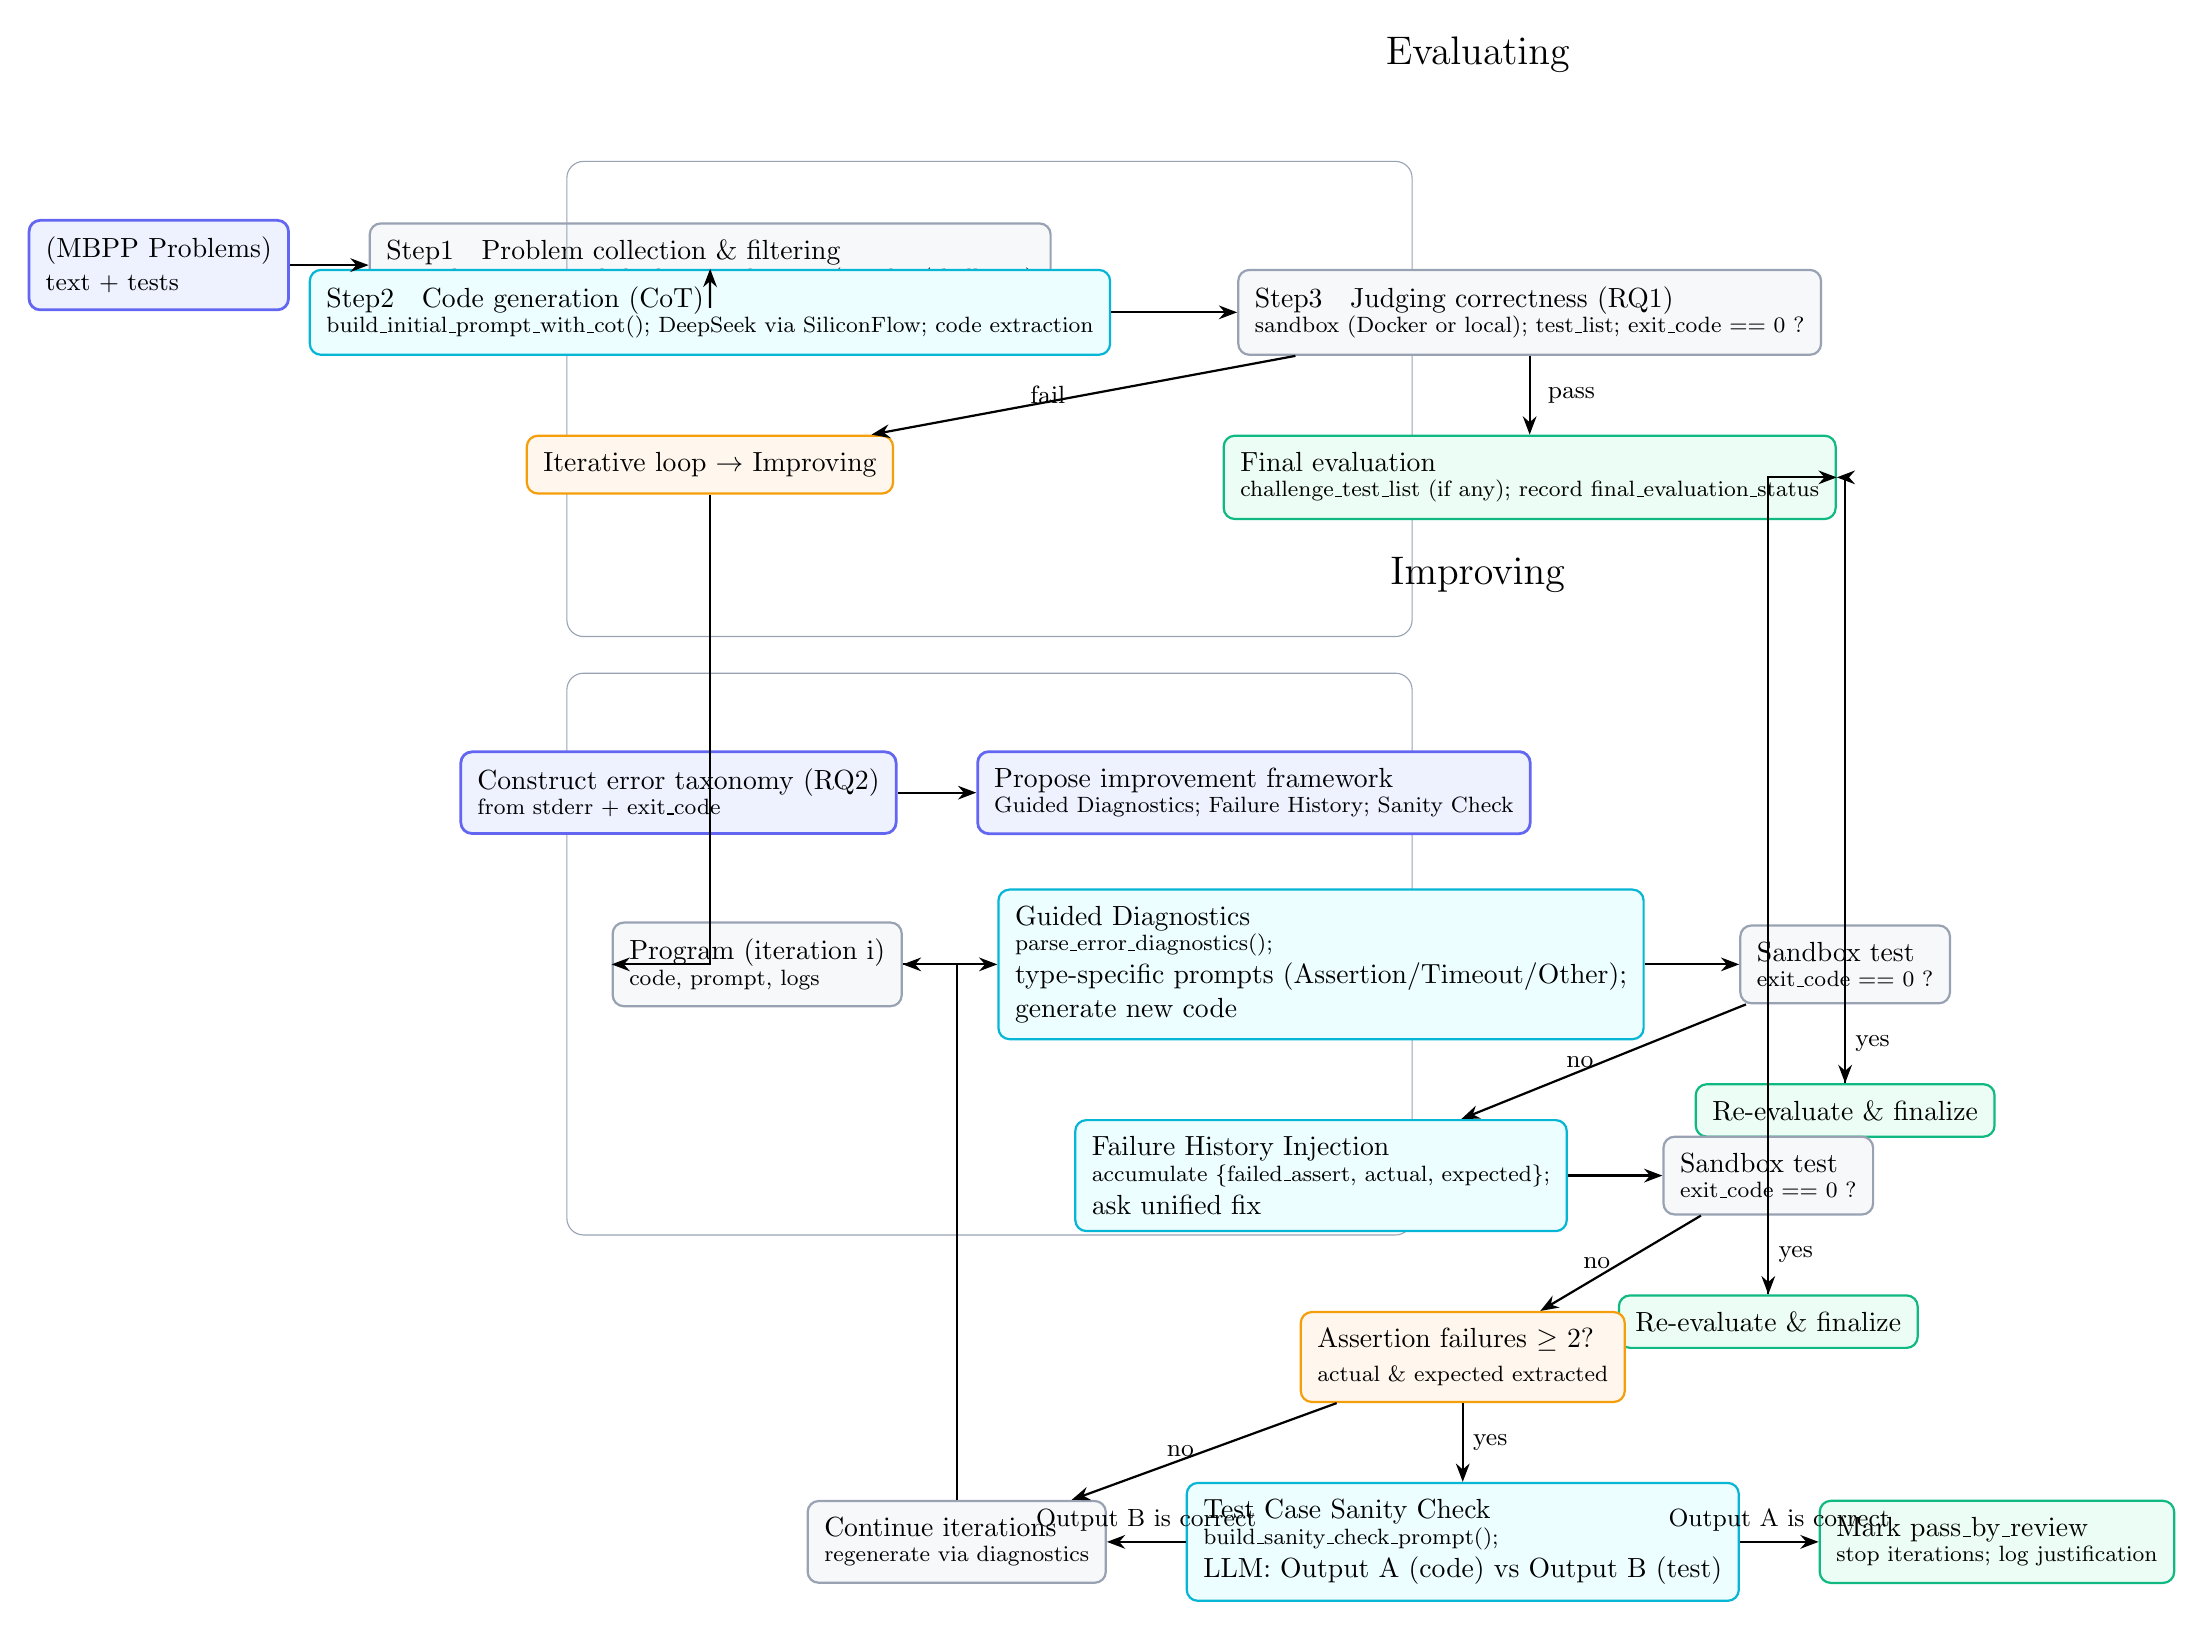
\begin{tikzpicture}[node distance=10mm and 10mm]
  % Inputs
  \node[key] (inp) {(MBPP Problems)\\\small text + tests};
  \node[stage, right=of inp] (step1) {Step1\quad Problem collection \& filtering\\[-1mm]\footnotesize normalize prompts; deduplicate; split tests (test\_list/challenge)};

  % Evaluating
  \node[draw=stagebd, rounded corners=6pt, fit={(5.3,1.2) (15.8,-4.6)}, label={[xshift=6.2cm,yshift=1.0cm]\Large Evaluating}] (evalbox) {};
  \node[proc] (g1) at (7.0,-0.6) {Step2\quad Code generation (CoT)\\[-1mm]\footnotesize build\_initial\_prompt\_with\_cot(); DeepSeek via SiliconFlow; code extraction};
  \node[stage, right=16mm of g1] (judge) {Step3\quad Judging correctness (RQ1)\\[-1mm]\footnotesize sandbox (Docker or local); test\_list; exit\_code == 0 ?};
  \node[ok, below=10mm of judge] (evalfin) {Final evaluation\\[-1mm]\footnotesize challenge\_test\_list (if any); record final\_evaluation\_status};
  \node[warn, below=10mm of g1] (toimp) {Iterative loop $\rightarrow$ Improving};

  \draw[flow] (inp) -- (step1);
  \draw[flow] (step1) -- (g1);
  \draw[flow] (g1) -- (judge);
  \draw[flow] (judge) -- node[right, xshift=1mm]{\small pass} (evalfin);
  \draw[flow] (judge) -- node[left, xshift=-1mm]{\small fail} (toimp);

  % Improving
  \node[draw=stagebd, rounded corners=6pt, fit={(5.3,-5.3) (15.8,-12.2)}, label={[xshift=6.2cm,yshift=0.9cm]\Large Improving}] (impbox) {};
  \node[key] (tax) at (6.6,-6.7) {Construct error taxonomy (RQ2)\\[-1mm]\footnotesize from stderr + exit\_code};
  \node[key, right=10mm of tax] (frm) {Propose improvement framework\\[-1mm]\footnotesize Guided Diagnostics; Failure History; Sanity Check};
  \draw[flow] (tax) -- (frm);

  \node[stage, below=11mm of tax, xshift=10mm] (prog) {Program (iteration i)\\[-1mm]\footnotesize code, prompt, logs};
  \node[proc, right=12mm of prog] (diag) {Guided Diagnostics\\[-1mm]\footnotesize parse\_error\_diagnostics();\\type-specific prompts (Assertion/Timeout/Other);\\generate new code};
  \node[stage, right=12mm of diag] (sbx1) {Sandbox test\\[-1mm]\footnotesize exit\_code == 0 ?};
  \node[ok, below=10mm of sbx1] (ok1) {Re-evaluate \& finalize};
  \node[proc, below=10mm of diag] (hist) {Failure History Injection\\[-1mm]\footnotesize accumulate \{failed\_assert, actual, expected\};\\ask unified fix};
  \node[stage, right=12mm of hist] (sbx2) {Sandbox test\\[-1mm]\footnotesize exit\_code == 0 ?};
  \node[ok, below=10mm of sbx2] (ok2) {Re-evaluate \& finalize};
  \node[warn, below=10mm of hist, xshift=18mm] (chk) {Assertion failures $\ge$ 2?\\\footnotesize actual \& expected extracted};
  \node[proc, below=10mm of chk] (sc) {Test Case Sanity Check\\[-1mm]\footnotesize build\_sanity\_check\_prompt();\\LLM: Output A (code) vs Output B (test)};
  \node[ok, right=10mm of sc] (pbr) {Mark pass\_by\_review\\[-1mm]\footnotesize stop iterations; log justification};
  \node[stage, left=10mm of sc] (cont) {Continue iterations\\[-1mm]\footnotesize regenerate via diagnostics};

  \draw[flow] (toimp) |- (prog);
  \draw[flow] (prog) -- (diag);
  \draw[flow] (diag) -- (sbx1);
  \draw[flow] (sbx1) -- node[right]{\small yes} (ok1);
  \draw[flow] (sbx1) -- node[left]{\small no} (hist);
  \draw[flow] (hist) -- (sbx2);
  \draw[flow] (sbx2) -- node[right]{\small yes} (ok2);
  \draw[flow] (sbx2) -- node[left]{\small no} (chk);
  \draw[flow] (chk) -- node[left]{\small no} (cont);
  \draw[flow] (chk) -- node[right]{\small yes} (sc);
  \draw[flow] (sc) -- node[above]{\small Output A is correct} (pbr);
  \draw[flow] (sc) -- node[above]{\small Output B is correct} (cont);
  \draw[flow] (cont) |- (prog);

  \draw[flow] (ok1) |- (evalfin);
  \draw[flow] (ok2) |- (evalfin);
\end{tikzpicture}
\end{document}


